\documentclass[11pt, oneside]{article}   	% use "amsart" instead of "article" for AMSLaTeX format
\usepackage{geometry}                		% See geometry.pdf to learn the layout options. There are lots.
\geometry{letterpaper}                   		% ... or a4paper or a5paper or ... 
%\geometry{landscape}                		% Activate for for rotated page geometry
%\usepackage[parfill]{parskip}    		% Activate to begin paragraphs with an empty line rather than an indent
\usepackage{graphicx}				% Use pdf, png, jpg, or eps� with pdflatex; use eps in DVI mode
								% TeX will automatically convert eps --> pdf in pdflatex		
\usepackage{amssymb}
\usepackage{amsmath}

\title{LU Decomposition}
%\author{The Author}
\date{}							% Activate to display a given date or no date

\graphicspath{{/Users/telliott_admin/Dropbox/Tex/png/}}

\usepackage{listings,relsize} 
\lstloadlanguages{R} 
\lstset{language=R,basicstyle=\smaller[1],commentstyle=\rmfamily\smaller, 
  showstringspaces=false,% 
  xleftmargin=4ex,literate={<-}{{$\leftarrow$}}1 {~}{{$\sim$}}1} 
\lstset{escapeinside={(*}{*)}}   % for (*\ref{ }*) inside lstlistings (S code) 
\begin{document}

\maketitle
%\section{}
% \subsection*{R code}
% \begin{lstlisting}  \end{lstlisting}
% \begin{center} 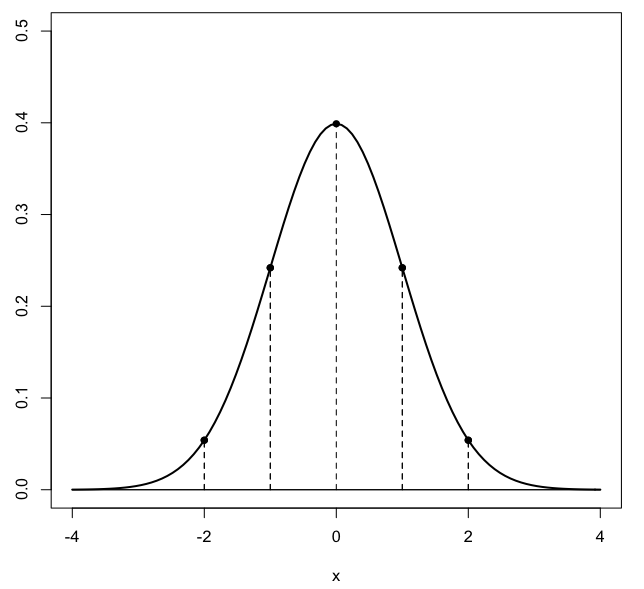
\includegraphics [scale=0.4] {gauss3.png} \end{center}
% \begin{bmatrix} a  &  b \\ c  &  d \end{bmatrix}
% \bigg |_

\large
\noindent
To find the "LU" decomposition of a matrix $A$ is to find
\[ A = LU \]
where $L$ is a "lower triangular matrix" and $U$ is an "upper triangular matrix."  What is meant is that $L$ has the form
\[
\begin{bmatrix} 
  a  &  0  &  0 \\ 
  b  &  c  &  0 \\
  d  &  e  &  f
\end{bmatrix} \ \ 
\]
Every entry \emph{above} the diagonal is 0.  Typically the entries of $L$ on the diagonal are $1$.
\[ L =
\begin{bmatrix} 
  1  &  0  &  0 \\ 
  b  &  1  &  0 \\
  d  &  e  &  1
\end{bmatrix} \ \ 
\]
$U$ is the reverse:  every entry \emph{below} the diagonal is 0.
The 2x2 version is about as simple as linear algebra can be.  Suppose we have
\[ 
A  =
\begin{bmatrix} 
  2  &  1  \\ 
  8  &  7  \\
\end{bmatrix}  \ \ 
\rightarrow \ \ 
U = 
\begin{bmatrix} 
  2  &  1  \\ 
  0  &  3  \\
\end{bmatrix}  \ \ 
\]
produced by elimination.  $U$ is upper triangular.  The matrix that can do this is
\[ 
E  =
\begin{bmatrix} 
  1  &  0  \\ 
  -4  &  1  \\
\end{bmatrix}  \ \ 
\]
\[ 
E A =
\begin{bmatrix} 
\ \   1  &  0  \\ 
  -4  &  1  \\
\end{bmatrix}  \ \ 
\begin{bmatrix} 
  2  &  1  \\ 
  8  &  7  \\
\end{bmatrix}  \ \ 
=
\begin{bmatrix} 
  2  &  1  \\ 
  0  &  3  \\
\end{bmatrix}  \ \ 
=
U
\]
So we have 
\[ EA = U \]
But we want
\[ A = LU \]
so clearly 
\[ E^{-1}EA = A = E^{-1}U = LU \]
\[ E^{-1} = L \]
For a 2x2 with one $E$ matrix it's easy
\[ 
E  =
\begin{bmatrix} 
\ \   1  &  0  \\ 
  -4  &  1  \\
\end{bmatrix}  \ \ 
\]
We use the standard method for 2x2.  Find $det(E)$, which is $1$.  If it were otherwise, we would multiply the result by $1/det$.  Switch the values at the $a$ and $d$ positions, and negate the others.
\[ 
E^{-1} =
\begin{bmatrix} 
  1  &  0  \\ 
  4  &  1  \\
\end{bmatrix}
\]
Check that we have it right
\[ 
EE^{-1} =
\begin{bmatrix} 
\ \   1  &  0  \\ 
  -4  &  1  \\
\end{bmatrix}  \ \ 
\begin{bmatrix} 
  1  &  0  \\ 
  4  &  1  \\
\end{bmatrix}
=
\begin{bmatrix} 
  1  &  0  \\ 
  0  &  1  \\
\end{bmatrix}  \ \ 
= I
\]
\[ 
LU =
\begin{bmatrix} 
  1  &  0  \\ 
  4  &  1  \\
\end{bmatrix}
\begin{bmatrix} 
  2  &  1  \\ 
  0  &  3  \\
\end{bmatrix}  \ \ 
=
\begin{bmatrix} 
  2  &  1  \\ 
  8  &  7  \\
\end{bmatrix}  \ \ 
= A
\]
Simple as that! 
An additional factorization could be done to bring the diagonal entries of $U$ out, like this
\[
\begin{bmatrix} 
  1  &  0  \\ 
  4  &  1  \\
\end{bmatrix}
\begin{bmatrix} 
  2  &  0  \\ 
  0  &  3  \\
\end{bmatrix}  \ \ 
\begin{bmatrix} 
  1  &  \frac{1}{2}  \\ 
  0  &  1  \\
\end{bmatrix}  \ \ 
= A
\]

\end{document}  